\documentclass[dvips,letterpaper,12pt]{report}
\usepackage[square,numbers]{natbib}
\usepackage{url}
\usepackage{thesis}
\usepackage{graphicx}
\usepackage{amsmath}
\begin{document}
\chapter{Introduction}

Augmented reality (AR) systems combine standard video inputs with computer-generated objects and
usually provide real-time interaction for the users. 
In general, an augmented reality system can be defined with the following properties \cite{azuma01} :
\begin{itemize}
\item Combination of real and virtual environment
\item Registration (alignment) of real and virtual objects
\item Real-time interaction
\end{itemize}
This concept was pioneered in the 1960s by an American computer scientist named Ivan Sutherland
who created the first head-mounted augmented reality
system with the help of one of his students \cite{azuma01}.

Combining virtual objects and annotations with real
world scenes has proved to be an effective way of conveying information about the surrounding environment to
the user and can be useful in many applications such as gaming, medical surgeries, tourism, and other entertaining, informative or instructional tasks.

Many mobile augmented reality systems have been built over the past decades, from touring machine in 1997 \cite{fei97} 
to google AR glasses which was announced in 2013 \cite{google}; however, most of these prototypes have remained as laboratory prototypes
due to certain difficulties and constraints of using them in practical applications. To name some of the most important constraints
we can refer to \cite{liv05}:
\begin{enumerate}
\item The requirement of having more advanced hardware and technology
\item Human factors in augmented reality 
\item Optimization of computational resources in order to provide a real-time interaction between the user and the system
\end{enumerate}

AR systems overlay 2D or 3D virtual objects on real scenes. Therefore, depending on the application, certain accuracy would be required for 
registeration of virtual and real objects. There are different approaches to obtain user's location and the position of other objects in the environment.
Tracking sensors such as gyroscope and accelerometer along with video sensors can provide information on the user's position and viewing orientation \cite{azum01}.
In order to find the position of the objects in the scene, a depth map of the surrounding environment at each time would be required. To obtain the depth of the 
objects in the scene several depth sensing technologies can be used such as 3D laser scanner, depth cameras or regular cameras. However, in order to have a mobile AR
system that is easy to carry around, the weight of the whole system will be more of a concern, hence, 3D laser scanners and depth cameras are not good choices for such systems.
Depth cameras, such as Kinect, or DS325 have certain limitation in viewing range (1m-5m) which would get worse in outdoor environments due to various types of noise. 
On the other hand, 3D laser scanners can
generate very accurate depth maps, but they are normally expensive and their price would range from 500\$ to 50,000\$. Therefore, among all these technologies, using several 
cameras to generate a depth map of the surrounding environment seems to be a more efficient approach for outdoor mobile augmented reality systems. {\newline}
However, using several cameras to get the depth map of the scene requires certain conditions to be met, geometrically and computationally. Many researchers have already looked into
this particular problem, i.e, finding the 3D position of the points in the scene from two or multiple views using regular cameras \cite{sze11}. Attempts of these researchers have resulted in
certain techniques in computer vision to find the depth of different points in an environment using one or more stereo pairs taken from slightly different points of view of the same scene.
These techniques are known as {\it Stereo Correspondence} or {\it Stereo Matching} in computer vision \cite{sze11}. Stereo matching has been one of the most sutdied subjects in computer vision for 
many years now and there are many solutions proposed by researchers to address this problem using different techniques; however, finding the corresponding pixels in stereo pairs with certain level of 
accuracy and in real-time for practical applications still remains a challenging task. {\newline}

% Motivation - Objective - Contributions %
Our motivation in this research is to study the possibility and usability of combining stereo vision approaches with AR systems considering the most important constraints that AR systems
normally come across, i.e., we would like to see whether using stereo vision
for obtaining 3D position of objects is potentially a good approach in an augmented reality application. A particular application that we are interested in for
our study is a 3D mobile augmented reality system in urban settings. In order to pursue our goal for this research, we have designed and implemented a testbed for evaluation of
stereo matching solutions based on specific criteria which will be thoroughly described in the next chapters.

In the system of our ineterst, the depth map generated from two or multiple camera views will be used as the depth source to determine the position of the objects in the scene when
overlaying virtual objects at different locations and depth levels in the real environment. For our research, we decided to narrow down our study to the effect of using stereo vision
on two of the most important constraints of an AR system mentioned earlier; {\it human factors} and {\it real-time interaction}. {\newline}
Human perception of depth can vary depending on the environment and under different circumstances. Many studies have focused on the evaluation of human perception of depth within different
criteria, such as virtual reality, and augmented reality which have recently attracted more attention. \textbf{REFERENCE}
These studies show that the viewer perception of depth
is inversely proportional to his distance from the object \cite{kru10,swa07,jer05,liv05}. For instance, in \cite{swa07} some experiments are designed to study and evaluate human
perception of absolute depth for an outdoor augmented reality application in urban settings. 
However, what we are more interested in is the human perception of relative depth in stereo vision. This metric can be estimated based on the ability to distinguish the depth of two different points
at a certain distance. The smallest depth difference between two points that can be detected in binocular vision is called stereoscopic acuity \textbf{REFERENCE}. More detail about
this metric will be provided in the next chapters.
Therefore, we have investigated and applied stereoacuity of human eyes in our evaluation in order to obtain the smallest detectable depth of 
objects in human binocular vision based on their distance from the observer.

Moreover, providing real-time interaction in an AR system for the user requires the processing time and update rate of the whole system to keep up idealy with the standard video frame rate, 
between 24fps and 
30fps. However, studies show that in practice to build a reasonable interactive augmented world the processing rate should not be less than half of the video frame rate  \textbf{NOTE: Search for more
valid reference} \cite{spe}. 
There are different approaches to speed up a system. Acceleration of a system is possible in two ways:
\begin{enumerate}
\item Using more advanced technology and hardware
\item More sophisticated and efficient software design
\end{enumerate}
However, having access to advanced technology and better hardware is not always feasible and even the most advanced technology have some limitation to their memory space and computional capability
which may not meet the requirement for some real-time applications. 
Therefore, we have decided to focus more on the second approach while designing our evaluation system which also looks into the 3rd most important property of
an AR system mentioned earlier, i.e, real-time user interaction. \newline 

One of the most important features that makes our evaluation unique and different from the others is that we have tailored the evaluation process of stereo matching algorithms for an augmneted 
reality system. Therefore, we have designed our evaluation testbed within this framework, while keeping in mind the most important properties and constrains of an AR system.
In order to address the speed factor in augmented reality systems we have decided to focus on certain regions of the scene rather than the whole image for generation and evaluation of 
depth values.  
This idea which originates from having a more efficient design for gaining speed up, 
also addresses the computational resources used during the process and may lead to significant system speed up.
It is also known that distinctive features such as the edges, either RGB or depth, in a scene play an important role for object detection and their corresponding depth perception in human visual
system \cite{sze11}.
\textbf {(REFERENCE)}
Therefore, in an augmneted reality application, wrong depth results, especially in those regions, which will lead to erroneous registeration of virtual and real objects, 
can be perceived and picked out easier by the human eyes. This may cause poor performance of the system and possibly faulty interaction between 
the user and the augmented world. 
Hence, in this research we have focused more on studying and evaluating the results of stereo correspondence algorithms in particular regions. Since the depth of the objects 
in a scene and their perception by human visual system are more important in the AR application of our interest, we have 
defined these regions to be depth edges and their surrounding region in the scene.
Our hypothesis is that the depth edges, which normally include object boundaries as well, are important depth cues for the user to perceive the depth of different objects in the scene. 
Moreover, inspection of the regions within a few pixels of the depth edges in the scene would also address the problem of occlusion and depth discontinuity, which are two of
the most challenging regions in stereo matching algorithms \cite{sch02}.
Finding correct depth values in these 
regions can lead to more accurate combination of virtual and real objects in the scene and therefore a more reasonable augmented world from the user point of view to interact with. \newline
\newline

Since our objective in this research is to study the combination of stereo vision and augmented reality systems, we have surveyed some of the existing approaches in stereo matching and the
related geometry for 3D reconstruction from stereo pairs. We will go through the related works and background more in the next chapter. 

To evaluate our proposition in this research, we have decided to assess two stereo matching alogirthms. These algorithms are as follow:
\begin{enumerate}
\item Semi-global stereo matching and mutual information by Hirschmuller \cite{hir08}
\item On building an accurate stereo matching system on graphics hardware \cite{mei11}
\end{enumerate}

The first algorithm by Hirschmuller has already been implemented in Open Source Computer Vision Library (OpenCV) \cite{sgbm}. Therefore, we have used its Opencv implementation that is 
called SGBM. On the other hand, there was no source code available for the second algorithm. So, we have used our own implementation of this solution in the evaluation process, both on CPU and GPU.

The reason we have chosen these two algorithms is that the first method, SGBM, has shown to generate acceptable results within 1-2 seconds on typical test images \cite{hir08} and 
its implementation in OpenCV library has also made its usage more common and easier in applications. The second algorithm, also known as ADCensus, was chosen since it has been designed in a way that
can be ported to graphics processing unit for accelartion and according to Middleburry evaluation benchmark it is currently ranked as one of the top algorithms for stereo matching \cite{mideval}.
It should also be noted that this solution uses better and more complicated approaches to do stereo matching which makes it superior to many other solutions. \newline
For our evaluation, we have used KITTI stereo training dataset as our stereo inputs \cite{kitti}. 
These images are more realistic and they have been taken from outdoor scenes under different circumstances 
and the ground truth disparity map is also provided for each of them which is useful in the evaluation process. KITTI Vision project also provides a benchmark and an evaluation table
for different stereo
matching algorithms assessed in real outdoor scenes which makes it more relevant and applicable to our interest in this research. 
AdCensus currently does not exist in their evaluation table which is another reason for us to use it in our evaluation.


\chapter{Background and Related Works}
Stereo vision is the concept of viewing a scene (object) in the real world from slightly different
viewpoints at the same time which results in stereo images. Using computer vision techniques, it is possible to extract depth information from stereo
images. This process is called {\it Stereo Matching} or {\it Stereo Correspondence} in computer vision,
which in fact leads to the construction of a
3D model of a scene from two or multiple views by finding corresponding pixels and therefore, their spatial movement within various views of the same scene \cite{sze11}.

Corresponding pixels in stereo images are the ones that represent the same point in the real
world. As it will be seen shortly in more detail, the amount of horizontal motion of such pixels
in stereo pairs, which is referred to as {\it disparity}, is inversely proportional to the
distance from the observee, i.e., depth; however,  estimation of the exact depth of the points requires some
other information as well, such as the position, and the calibration data of the cameras that took the pictures.
While the physical and geometrical approaches to this problem are well understood by researchers in the field, the process of finding the corresponding pixels correctly, yet efficiently
and measuring the disparity to generate a dense depth map still remains a challenging task. \newline

\section{Epipolar Geometry}
The basic geometry of stereo matching is described in more detail in this section. 
The epipolar geometry in stereo images is defined by the intersection between the image planes and any plane having the line between two camera centers, known as {\it baseline}, as axis. 
This geometry helps to understand the core idea of stereo matching algorithms and 3D model reconstruction from stereo images.
(\textbf {FIGURE  for epipolar planes similiar to the figure in multipleview geometry page240})
%\begin{figure}{h!}
%\centering
%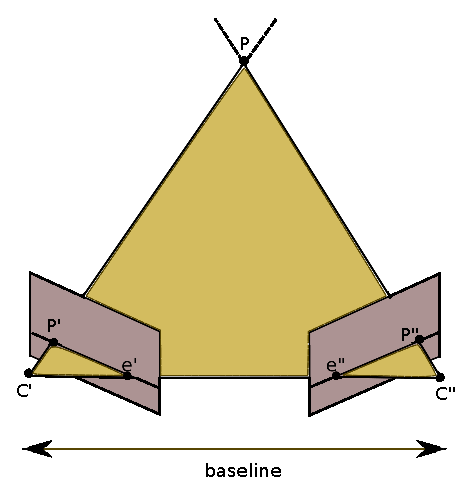
\includegraphics[width=1.5in,height=1.5in]{epipole}
%\end{figure}

If we consider a point P in space and project it back as P' and P'' with rays passing through each camera's centre
into the left and right image planes, there will be a common feature between all these points and the camera centres which serves as an important property while searcing for corresponding points
in stereo matching algorithms. Let us call the plane traversing all these points $\pi$.
Now, suppose that we only know the position of the point P' in the left image and want to find its correspondence, P'', in the right plane. According to the aformentioned property, P',
its correspondence and their projection in 3D space are all coplanar with camera centres. This plane, $\pi$, is defined by the line connecting two camera centres and 
the rays passing through P' and the left camera centre. Therefore, the point P'' would lie somewhere on the line created by the intersection of $\pi$ and the right image plane.
This line is in fact the back-projection in the right image plane of the ray passing through P'. This line is called the {\it epipolar line} corresponding to P'. Hence, in a stereo matching algorithm
we only need to search this line rather than the whole image in order to find the corresponding point for point P'.
In order to better understand the principal idea behind stereo matching algorithms, some fundamental concepts in epipolar geomtery must be fist introduced. 
Here, we explain these concepts briefly and an allustration of them is also provided in figure \textbf{FIGURE NUMER}.
\newline
The fundamental entities in epipolar geometry are as follow: \cite{hart2000}
\begin{itemize}
\item The \textbf{epipole}: The point of intesection between the baseline and each of the image planes is called the epipole. In other words, each epipole can be referred to as the image of one of
the camera centres in the other image plane.

\item The \textbf{epipolar plane}: Any plane containing the line between camera centres is called the epipolar plane. The collection of these planes is called an epipolar pencil. 

\item The \textbf{epipolar line}: The intersection of the epipolar plane and the image plane creates a line called epipolar line. The epipolar line always passes through the epipole in the 
image plane.
\end{itemize}

(\textbf{FIGURE HERE FOR EPIPOLAR GEOMETRY TERMS}) 
\newline 
Knowing the concepts in epipolar geometry helps to better understand how stereo correspondence algorithms work. Based on the description of epipolar geometry, 
we know that in order to find the correspondence of a particular point P' in the second image plane, first the corresponding epipolar line must be found. 
Therefore, there is a projective mapping from each point in the first image 
to its corresponding epipolar line in the second image, which can be represented as a matrix that is independant of the scene and is related to the camera's properties.\cite{hart2000} As it can be
seen in figure (\textbf{figure number}), mapping from point P' to its correspondence, P'', in the other image plane requires certain transformations; rotation and translation. However, in order
to make the scanning process for correspondences more efficient in stereo matching algorithms, 
it is better to have the input image pairs warped first, i.e., {\it rectified}. The best way to accomplish this task is to
rotate both cameras first so that their optical axis, the line passing through the camera centre which is perpendicular to the image plane, are parallel to each other; 
i.e., their optical axis is perpendicular to the baseline. Furthermore, it is necessary to have the camera's {\it y} axis perpendicular to the optical axis. After these two steps,
corresponding epipolar lines will be horizontal which constrains the process of searching for the corresponding points. 
In this model, the disparity for points at infinity is also equal to 0.\cite{sze11}
The relation between particular geometrical parameters through which the depth of a certain point in 3D space is obtained, can be clearly defined base on the aforementioed rectified model. 
This relation is presented as follows:
\begin{center}
$d = f\frac{B}{Z}$
\end{center}
where f is the {\it focal length} measured in pixels, B is the {\it baseline}, Z is the {\it 3D depths}, and d is {\it disparity}. The relationship between corresponding pixels in the left
and right images according to disparity {\it d} is also as follows:
\begin{center}
${P}''_{x}={P}'_{x}+d(x,y)$

${P}''_{y} = {P}'_{y}$
\end{center}
Therefore, based on the aforementioned formulas, the depth of points in 3D space can be easily calculated after finding the corresponding pixels in multiple views and consequently their
disparities. \cite{bol87,oku93,sch02}

\section{Stereo Correspondence Algorithms}
A survey of the field shows that the algorithms which address stereo correspondence problem can be roughly divided into two main classes \cite{sch02}. These classifications are commonly known as:
\begin{enumerate}
\item Sparse Correspondence Algorithms
\item Dense Correspondence Algorithms 
\end{enumerate}

In this section, we are going to briefly describe the important specifications of the algorithms belonging to each of these two categories.
\subsection{Sparse Correspondence Algorithms}
Sparse correspondence algorithms, also known as feature-based algorithms, are the early stereo matching methods. In this type of methods, particular features in an image, such as edge 
points, line segments, or other significant features are extracted and therefore, the search for corresponding pixels is only applied to these regions. Consequently, algorithms of this
type result in a sparse disparity map \cite{matt89,hsie92, sze11}. The introduction of feature-based algorithms has mainly been motivated by three important reasons \cite{sze11}:
\begin{itemize}
\item Limitation in computational resources.
\item Constraint of the searching area in order to find more reliable matches.
\item Images with different illumination, where edges or some other particular features preserves their photometric properties and therefore, are the only regions reliable enough to 
be used for correspondence search.
\end{itemize}

\subsection{Dense Crrespondence Algorithms}
Unlike feature-based methods, dense correspondence algorithms try to find the
corresponding pixels in the whole image, and therefore, result in a dense disparity map. Most recent algorithms and studies have focused on this class of algorithms since many applications 
nowadays, such as image-based rendering, modeling, or augmented reality require a dense depth map of the scene. However, this class of algorithms face many challenges that need to be properly
addressed, such as finding the depth values in textureless areas, depth discontinuities, and occluded regions.

Dense correspondence algorithms can be classified in two groups based on how they assign
disparities to pixels:
\begin{enumerate}
\item Local approaches
\item Global approaches
\end{enumerate}

\textbf{Local Approaches}
\newline
Local methods tend to find the disparity of each pixel based on its local neighboring pixels. In
other words, the disparity of a pixel is calculated in a finite window, based on the intensity values
its of neighboring pixels in the same window \cite{sch02}.

These methods make an implicit smoothness assumption for the pixels in the search
window, and therefore, assign the same disparity to all the pixels belonging to the same window which could result in incorrect disparity values in slanted surfaces or
depth discontinuities \cite{hirsch02}. This assumption can be considered as one of the major drawbacks of local methods.
Another drawback of local methods is their dependency on the window size \cite{sch02}. A fixed window size can raise certain problems in these algorithms:
\begin{enumerate}
\item If too large of a window size is considered, due to aforementioned smoothness assumption, the algorithm may result in blurry object boundaries and inaccuracy near depth discontinuities.
\item If the window size chosen is too small, the disparity values will be less accurate since little information has been considered for 
finding the correspondences of pixels in the image.
\end{enumerate}

However, a significant advantage of using local approaches is their high speed in finding disparity results.\newline

\textbf {Global Approaches}
\newline
Unlike local approaches, in global methods the disparity of a pixel depends on the information in
the whole image. Global methods usually contain an optimization step of a global energy
function. In this class of algorithms, an optimal disparity value for each pixel is sought that lead to minimization of a global cost
function that normally combines a data term with an explicit smoothness assumption in form of \cite{roy98,bobi99,boyk01}:

\begin{center}
$E(d)=E_{data}(d)+\lambda E_{smooth}(d)$
\end{center}
The term $E_{data}$ normally represent the difference in the intensity of the corresponding pixels and is denoted as follows:

\begin{center}
$E_{data}(d) = \sum_{(x,y)}C(x,y,d(x,y))$
\end{center}

where C is the matching cost. The matching cost function can have various definitions depending on the algorithm; however, it is normally defined as sum of absolute difference 
between the intesity of the corresponding pixels in two images \cite{sch02}.

Due to the existence of the smoothness term, $E_{smooth}$, neighboring pixels tend to have similar disparity values. $\lambda$ is also a weight factor that can vary depending 
on the implementation of the global function in the algorithm \cite{sze11}.


The major drawback of global approaches is the high usage of computational resourses and the low speed in finding the matches. However, they usually result in more accurate disparity values
\cite{hirsch02,sze11}. 



\bibliographystyle{plain}
\bibliography{reference} 
\end{document}
